
\subsection{研究背景}

\subsubsection{内存与显存数据传输优化的意义}

在一般的GPU硬件加速的程序应用场景中,内存到显存的数据传输是不可避免的,Chris Gregg等人在论文Where is the Data? Why You Cannot Debate CPU vs. GPU Performance Without the Answer\cite{Where-is-the-Data}里面以十多项常见的GPU应用程序为benchmark,通过测试和分析不同数据规模下的benchmark运行效率发现内存与显存之间的数据传输几乎对所有的GPU应用程序运行性能都有着十分重要的影响。特别是在大数据输入集下,内存与显存传输的时间开销最高可以达到GPU计算时间开销的50多倍。由此我们可以得到结论:内存与显存的数据传输是影响GPU应用程序性能的重要的因素。


\subsubsection{CPU与GPU的访存机制}

我们首先介绍以下GPU的访存机制。GPU使用的内存分为两个部分,一部分是显卡自带的显存称为VRAM(Vedio RAM),另一部分是系统主存(即CPU端内存)也称为GTT内存。为了实现GPU同时使用VRAM内存和GTT内存最简单的方法就是将这两片内存统一编址,VRAM是显卡自带的内存,它的地址一定是连续的,但是不连续的GTT内存如果要统一编址,那么一定需要通过建立页表映射关系,这个页表也就是GTT(graphics translation table, 地址转换表)。

和CPU的地址类似,GPU直接使用的地址被称为“GPU虚拟地址”,经过查页表转化之后的地址称为“GPU物理地址”,也就是GPU最终真实访问的地址,其中GPU的虚拟地址和物理地址转换过程如图\ref{fig:gpu-mmu}所示:对于属于GTT的虚拟地址,通过查找GPU页表找到真实的PCI地址,然后通过PCI地址访问系统主存;对于属于VRAM的虚拟地址则无须页表转换直接在VRAM内寻址。

\begin{figure}[H] 
  \centering
  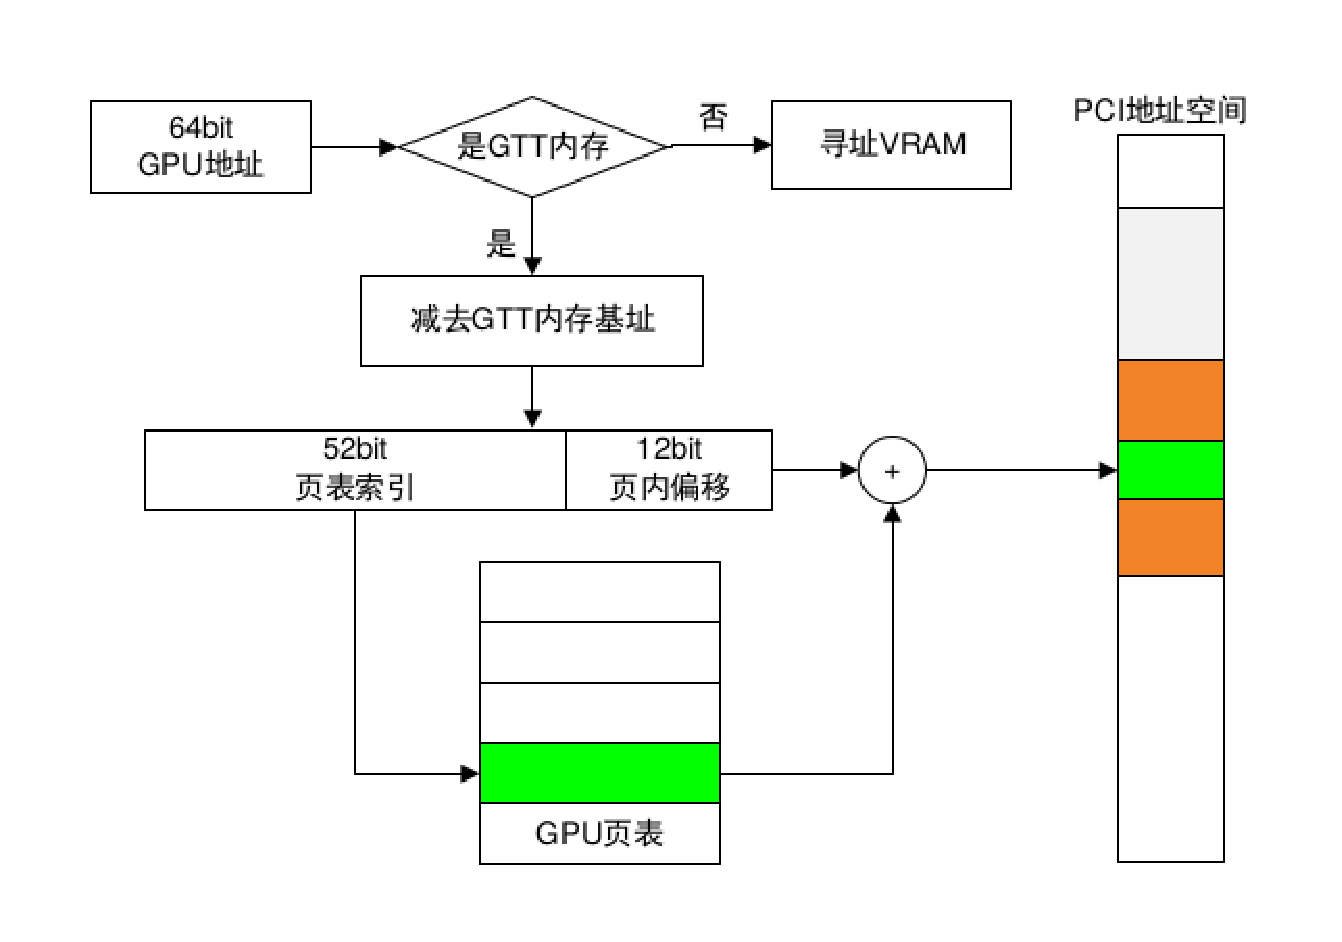
\includegraphics[width=12cm,height=8cm]{figures/chap03/gpu-mmu}
  \caption{GPU的内存访问机制}
  \label{fig:gpu-mmu}
\end{figure}

与此同时,CPU使用的内存就复杂的多了,CPU通过MMU单元将虚拟地址转化成实际的物理地址,这些物理地址有的是系统主存的地址,有些是外接设备的地址,其中就包括GPU的自带显存VRAM地址。通过下图\ref{fig:cpu-gpu-mm}可以看到,CPU和GPU均能自有访问系统内存和显卡内存VRAM。

\begin{figure}[H] 
  \centering
  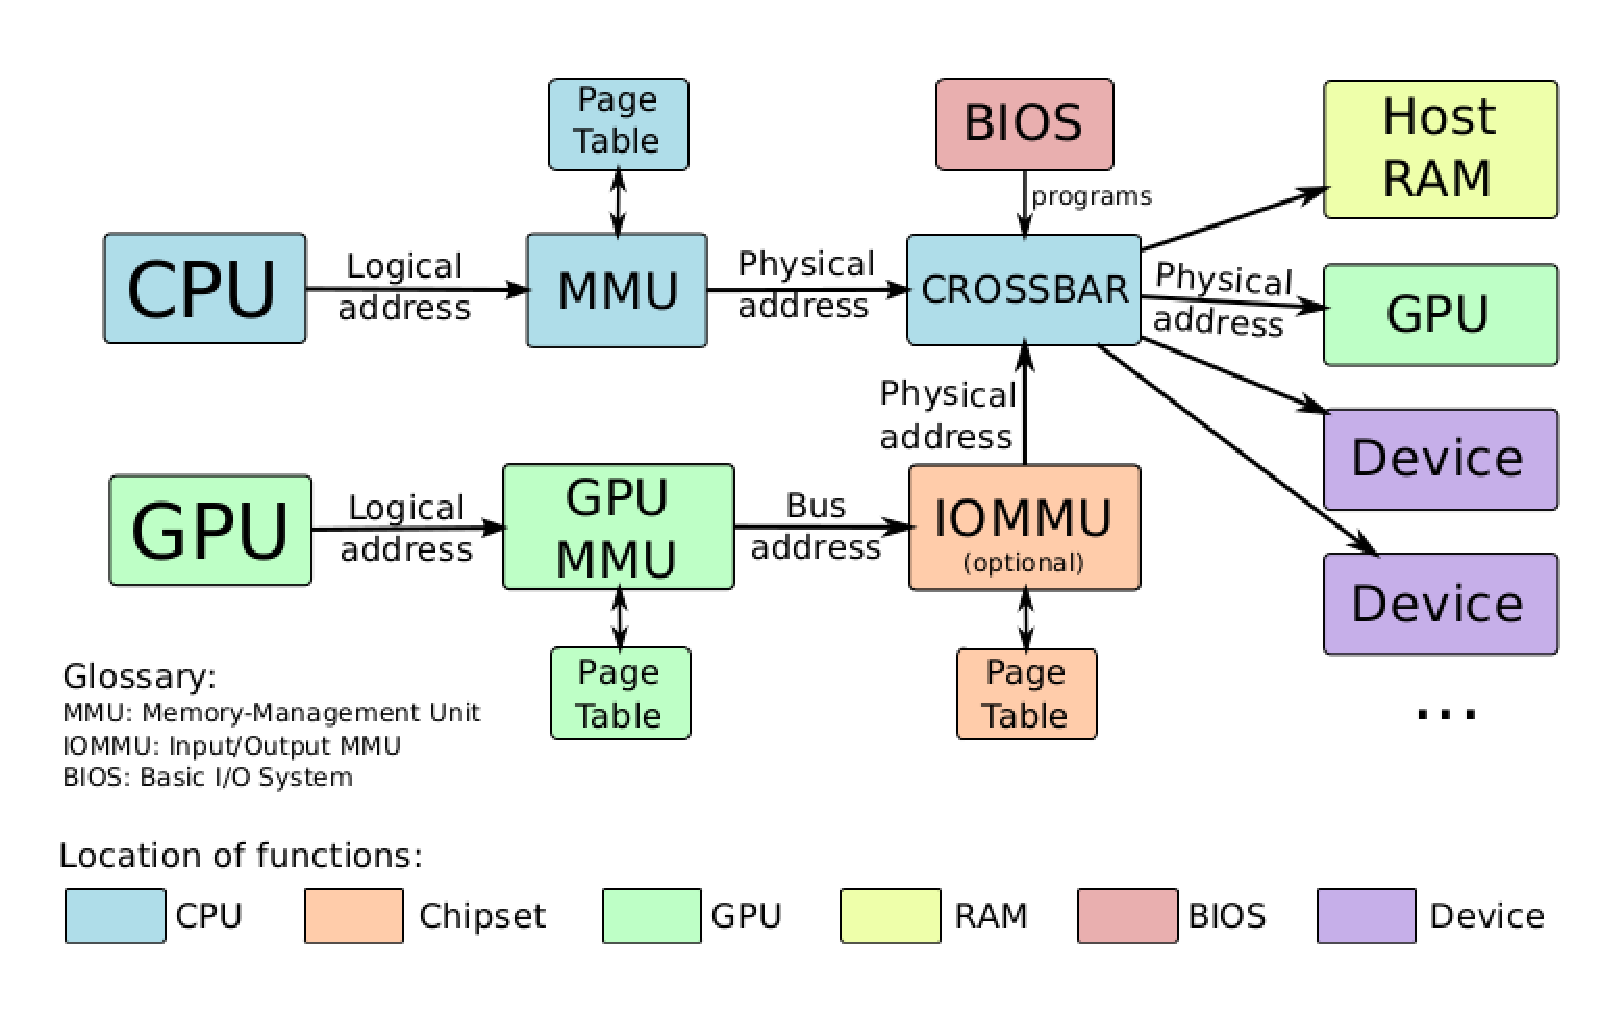
\includegraphics[width=12cm,height=8cm]{figures/chap03/cpu-gpu-mm}
  \caption{CPU与GPU内存请求回路}
  \label{fig:cpu-gpu-mm}
\end{figure}

\subsubsection{龙芯平台下四种内存传输的性能分析}

从前面我们可以看到存在着四种内存传输,它们分别是: 系统内存到系统内存、系统内存到显存、显存到系统内存和显存到显存。这里本文以龙芯3A搭载Radeon R600显卡平台为例测试并研究四种内存访问模式的性能。得到相关数据如下图\ref{fig:memcpy-performance}所示:

\begin{figure}[H] 
  \centering
  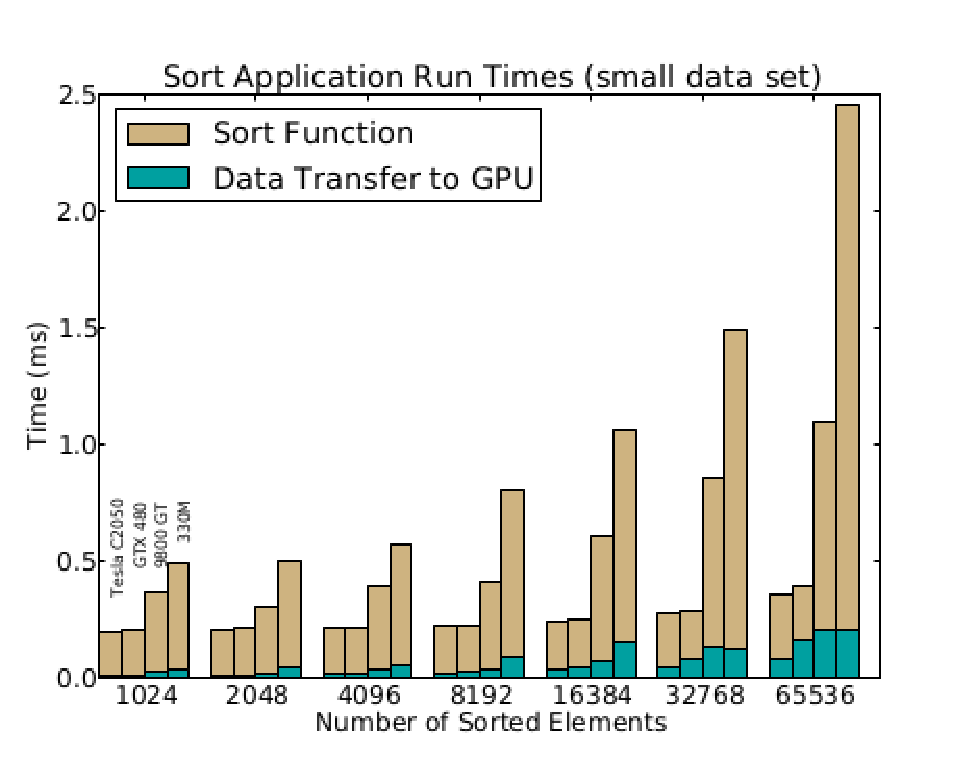
\includegraphics[width=12cm,height=8cm]{figures/chap03/memcpy-performance}
  \caption{龙芯平台四种访存模式性能分析}
  \label{fig:memcpy-performance}
\end{figure}

通过上图\ref{fig:memcpy-performance}我们可以发现XXXX

\subsection{Mesa3D图形库CPU与GPU访存行为分析}

在Mesa3D图形库的实现中,CPU端在初始化过程中会创建顶点对象缓存区,而这些顶点对象缓存区是创建在VRAM之上的,然后通过内存映射的方式映射成CPU端虚拟地址进行访问。在上层程序需要使用Mesa3D进行图形绘制时候,Mesa3D会将绘制相关的顶点数据拷贝到顶点对象缓存区中,即发生了CPU端内存到显存的拷贝,整个过程是同步实现的,即需要占用CPU的指令周期。当GPU接受到绘制命令和相关顶点数据准备好时候,GPU就开始内部的硬件图形加速渲染管线进行图形渲染,并将渲染结果放置到显存的framebuffer中以待显示。这里面顶点数据和绘制命令也不是一次性完成的,可能会分很多周期完成,这里以svPerfGL测试集里面的顶点数组模式作为测试对象,测试数据并绘制成下图\ref{fig:mesa3d-data-transfer}的CPU/GPU工作时序图。

\begin{figure}[H] 
  \centering
  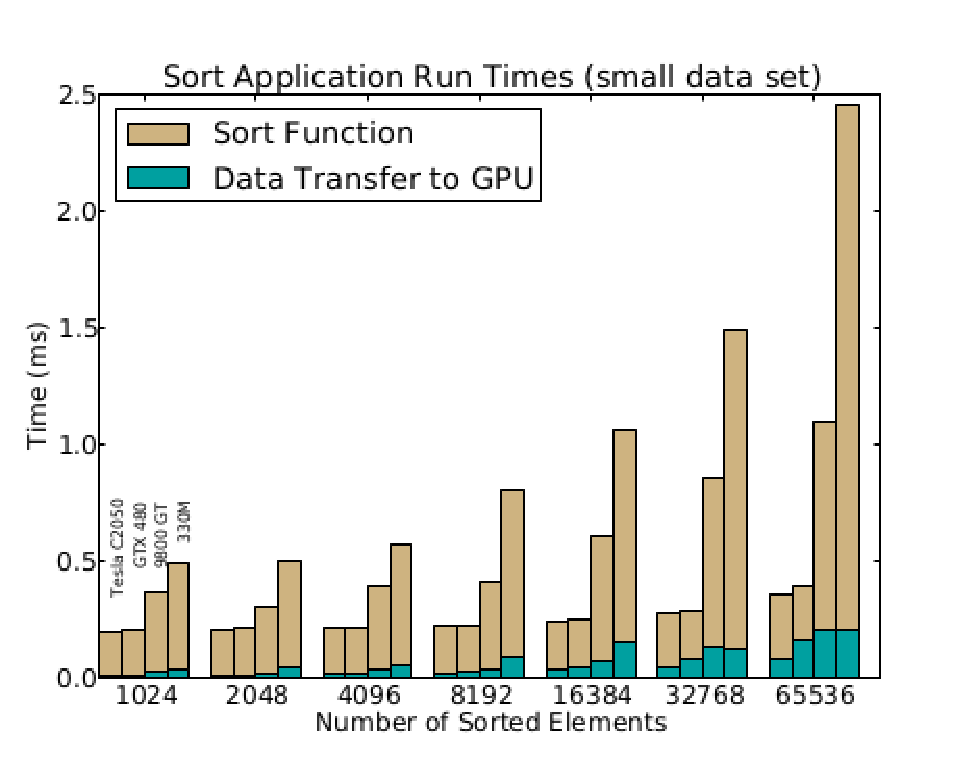
\includegraphics[width=10cm,height=6cm]{figures/chap03/mesa3d-data-transfer}
  \caption{svPerfGL测试集顶点数组模式CPU/GPU工作时序图}
  \label{fig:mesa3d-data-transfer}
\end{figure}

通过上面的时序图我们可以看到以下几点:

\begin{itemize}
\item{}数据传输部分是由CPU负责的,占用CPU的执行周期,而且传输时间较慢。
\item{}GPU每次在接受完数据之后就能很快的执行完渲染流程,其他大部分时间都处于等待数据准备的空闲状态。
\end{itemize}

\subsection{Mesa3D图形库CPU与GPU访存优化}

针对Mesa3D图形库实际的访存特点,本文从访存策略与拷贝效率这两个方面提出了相应的优化方案。

\subsubsection{CPU与GPU访存策略的优化}
从上面图\ref{fig:mesa3d-data-transfer}我们知道,由于CPU端内存到显存的数据拷贝效率低下,导致占用了大量的CPU执行周期,使得CPU执行时间占比过大,而GPU相对执行时间过少。为了改变这一状况,如下图\ref{fig:vbo-gtt}我们可以把顶点数据缓冲区创建在系统内存之上,CPU只需简单的系统内存内部搬运数据,而GPU则通过GTT的方式访问顶点数据缓冲区然后进行图形硬件渲染。

\begin{figure}[H] 
  \centering
  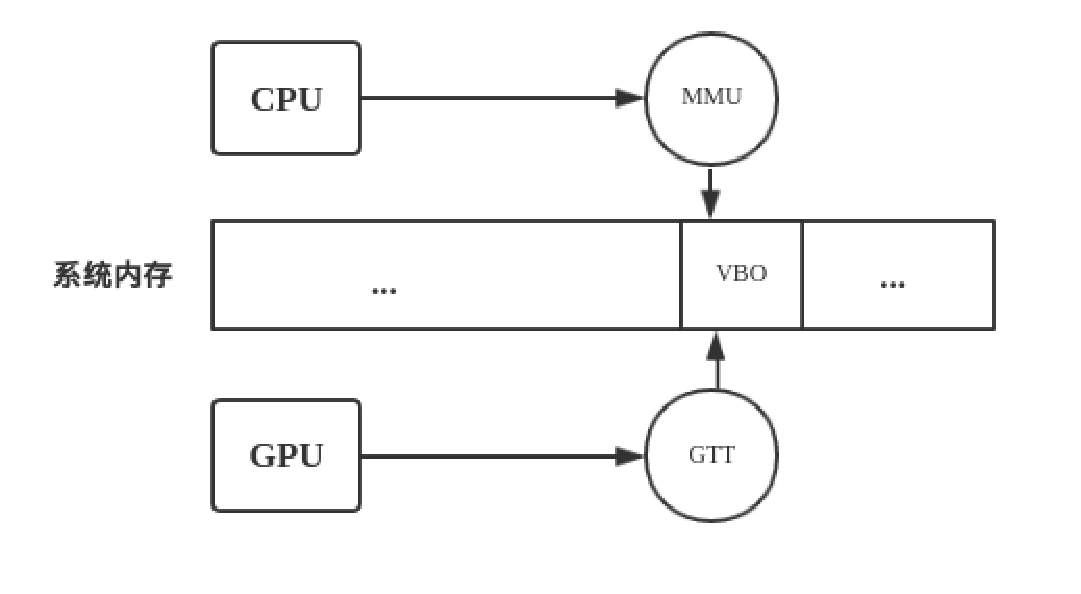
\includegraphics[width=10cm,height=6cm]{figures/chap03/vbo-gtt}
  \caption{Mesa3D图形库CPU与GPU改进后访存策略}
  \label{fig:vbo-gtt}
\end{figure}

虽然这样之后,GPU渲染时候的数据访问效率会降低,但是由于本身GPU工作负担小于CPU,所以整个CPU和GPU的并行程度提高了,还是以svPerfGL的顶点数组模式为例,测试改进后的效果如图\ref{mesa3d-data-transfer-gtt}所示。

\begin{figure}[H] 
  \centering
  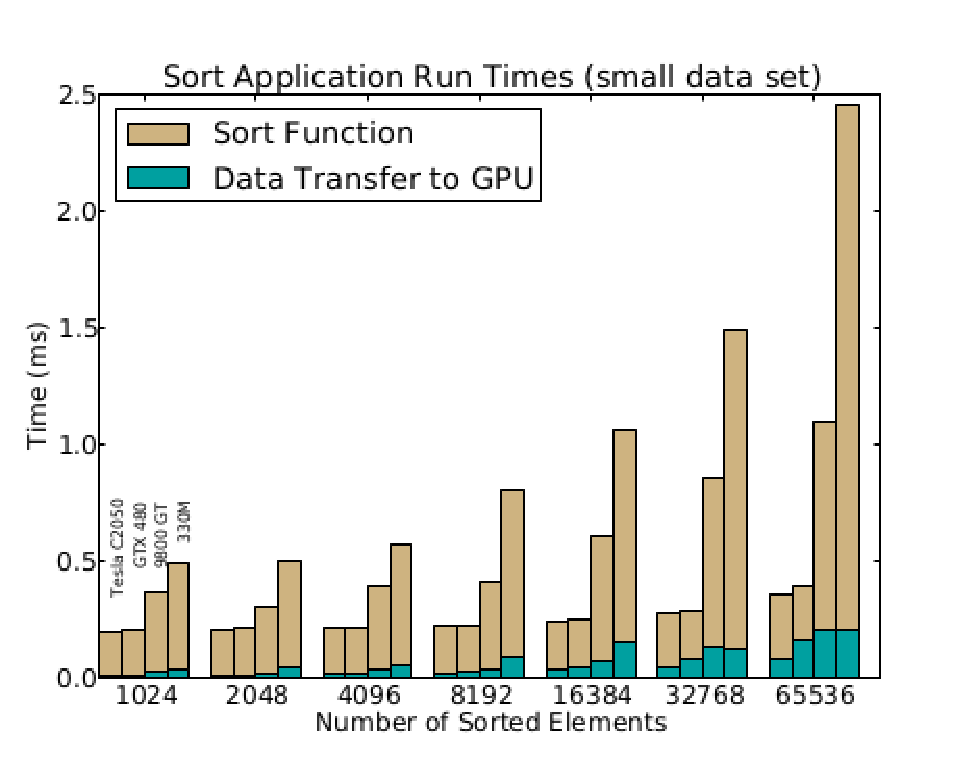
\includegraphics[width=10cm,height=6cm]{figures/chap03/mesa3d-data-transfer}
  \caption{svPerfGL测试集顶点数组模式CPU/GPU工作时序图}
  \label{fig:mesa3d-data-transfer-gtt}
\end{figure}

通过上图\ref{fig:mesa3d-data-transfer-gtt}可以看到XXXX

\subsubsection{CPU与GPU拷贝效率的优化}

在前一节的改进访存策略之后,我们可以通过提高拷贝效率来改进CPU与GPU的数据传输性能。由于CPU端向GTT的数据拷贝大多都是单精度浮点数据的拷贝,所以我们可以通过龙芯平台特有的宽位访存指令来提高拷贝效率。

\textbf{龙芯扩展宽位访存指令}: 龙芯平台为了自身发展的需求,通过龙芯指令系统融合技术\cite{loongson-merge},专门开发了一些宽位访存指令,诸如本文使用到的128bit浮点访存指令GSLQC1和GSSQC1可以实现128bit的浮点数据存取。



